\documentclass[tikz, border=10pt]{standalone}
\usepackage{helvet} % Set font to Helvetica
\renewcommand{\familydefault}{\sfdefault} % Make sans-serif the default
\usepackage[T1]{fontenc}

\usepackage{tikz}
\usetikzlibrary{shapes.geometric, arrows.meta, positioning, chains}

\begin{document}

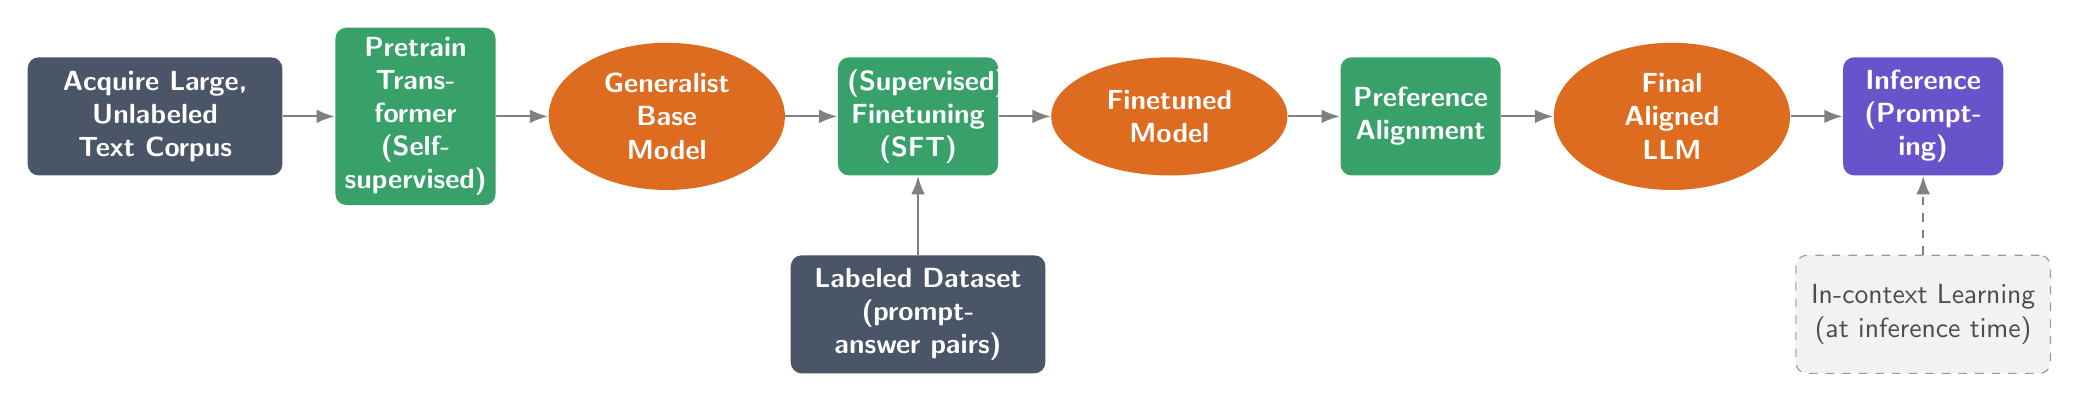
\begin{tikzpicture}[
    node distance=1.5cm and 0.66cm,
    start chain=main going right,
    font=\sffamily, % Apply sans-serif font to all nodes
    % MODERN STYLES: Flat, geometric, high-contrast
    base/.style={
        rectangle,
        text width=1.8cm,
        minimum height=1.5cm,
        align=center,
        text=white,
        font=\sffamily\bfseries,
        rounded corners=4pt,
        draw=none
    },
    data/.style={
        base,
        fill={rgb,255:red,74; green,85; blue,104}, % Slate Gray
        text width=3cm
    },
    process/.style={
        base,
        fill={rgb,255:red,56; green,161; blue,105} % Green
    },
    model/.style={
        base,
        shape=ellipse,
        minimum width=3cm,
        fill={rgb,255:red,221; green,107; blue,32} % Orange
    },
    final/.style={
        base,
        fill={rgb,255:red,104; green,83; blue,203} % Indigo
    },
    side/.style={
        rectangle,
        text width=3cm,
        minimum height=1.5cm,
        align=center,
        font=\sffamily,
        rounded corners=4pt,
        draw=black!40,
        dashed,
        fill=black!5,
        text=black!70
    },
    arrow/.style={
        -Latex,
        thick,
        draw=black!50
    }
]

% Place nodes on the main chain
\node[data, on chain] (corpus) {Acquire Large, Unlabeled Text Corpus};
\node[process, on chain] (pretrain) {Pretrain Transformer (Self-supervised)};
\node[model, on chain] (base_model) {Generalist Base Model};
\node[process, on chain] (sft) {(Supervised) Finetuning (SFT)};
\node[model, on chain] (tuned_model) {Finetuned Model};
\node[process, on chain] (align) {Preference Alignment};
\node[model, on chain] (final_model) {Final Aligned LLM};
\node[final, on chain] (inference) {Inference (Prompting)};

% Place side nodes, repositioned for horizontal layout
\node[data, below=of sft, yshift=0.5cm] (labeled_data) {Labeled Dataset (prompt-answer pairs)};
\node[side, below=of inference, yshift=0.5cm] (icl) {In-context Learning (at inference time)};

% Draw arrows for the main chain
\begin{scope}[on chain]
    \draw[arrow] (corpus) -- (pretrain);
    \draw[arrow] (pretrain) -- (base_model);
    \draw[arrow] (base_model) -- (sft);
    \draw[arrow] (sft) -- (tuned_model);
    \draw[arrow] (tuned_model) -- (align);
    \draw[arrow] (align) -- (final_model);
    \draw[arrow] (final_model) -- (inference);
\end{scope}

% Arrows for side nodes, adjusted for new positions
\draw[arrow] (labeled_data.north) -- (sft.south);
\draw[arrow, dashed] (icl.north) -- (inference.south);

\end{tikzpicture}

\end{document}

